\documentclass[11pt, aspectratio=169]{beamer}

% --- Core Packages for Modern Documents ---
\usepackage{fontspec}      
\usepackage{unicode-math}
% \usepackage{xeCJK}         
\usepackage{graphicx}      
\usepackage{minted}
\usepackage{setspace}
% \usepackage{tipa}
\usepackage{kotex}
\usepackage{graphicx}
\usepackage{tikz}
\usepackage{multicol}
\usepackage{hyperref}
\usepackage{emoji}

\usetikzlibrary{
    shapes.geometric, % 다양한 도형 사용
    arrows.meta,      % 화살표 스타일 설정
    positioning       % 노드 위치 선정
}

% \xeCJKsetup{CJKspace=true}

% --- Font Setup ---
\setsansfont{Noto Sans KR} %Noto Sans KR
\setmainfont{Noto Serif KR}
\setmonofont{D2Coding}

\setmainhangulfont{Noto Sans KR}
\setsanshangulfont{Noto Serif KR}
\setmonohangulfont{D2Coding}

% \setCJKsansfont{Noto Sans KR}  %나눔바른고딕 옛한글
% \setCJKmainfont{Noto Serif KR}
% \setCJKmonofont{D2Coding}

\setmathfont{Latin Modern Math}

\newfontfamily{\tnrfont}{Times New Roman}
\newcommand{\texttnr}[1]{{\tnrfont #1}}

\mode<presentation>
{
  \usetheme{default}      % or try Darmstadt, Madrid, Warsaw, Marburg...
  \usecolortheme{dove} % or try albatross, beaver, crane, dove...
  \usefonttheme{default}  % or try serif, structurebold, ...
  \setbeamertemplate{navigation symbols}{}
  \setbeamertemplate{caption}[numbered]
} 

\AtBeginSection[]{
  \begin{frame}
    \vfill % Vertically center the title
    \centering
      \usebeamerfont{title}\insertsectionhead\par
    \vfill
  \end{frame}
}

\renewcommand{\arraystretch}{1.3} % Set row height for ALL tables in the document to 1.5x

\definecolor{Highlight}{HTML}{FFF2CC} % A soft yellow

\definecolor{MonokaiBackground}{HTML}{272822}
\definecolor{blocktitle}{HTML}{7A8B5D}
\definecolor{blockbody}{HTML}{F0E085}
\definecolor{normaltext}{HTML}{E5E8D5}
\definecolor{structure_color}{HTML}{D1E1E8}

\setbeamercolor{normal text}{bg=normaltext, fg=black}
\setbeamercolor{structure}{bg=structure_color, fg=black}

\setbeamercolor{block title}{bg=blocktitle, fg=white}
\setbeamercolor{block body}{bg=blockbody, fg=black}
\setbeamertemplate{footline}{
  \hfill % Pushes the content to the right
  \usebeamercolor{page number in head/foot}
  \usebeamerfont{page number in head/foot}
  \insertframenumber{} / \inserttotalframenumber
  \hspace*{2ex} % Adds a little padding from the right edge
}

\setminted{
    style=default, % dracula, native, monokai...
    linenos,       % Show line numbers
    frame=lines,   % Draw a thin frame around the code
    framesep=2mm,
    xleftmargin=6pt,
    breaklines=true
}

% 제목 정보
\title{언어의 이해}
\subtitle{1강. 언어와 언어학}
\author{김미경}
\date{2025.9.3}

\begin{document}

% 제목 슬라이드
\frame{\titlepage}

% 목차
\begin{frame}[t]{목차}
\tableofcontents
\end{frame}

\section{언어, 언어학, 언어학자}

\begin{frame}[t]{언어의 두 가지 의미}
  \begin{block}{구체적, 개별적 `언어'}
    “그 사람은 언어 능력이 뛰어나다” = 할 줄 아는 외국어가 많다
    \begin{itemize}
      \item 한국어, 영어, 중국어, 일본어, 프랑스어 등
      \item 특정 언어 공동체가 사용하는 개별 언어
    \end{itemize}    
  \end{block}
  \begin{block}{추상적 `언어'}
    “우리 애는 언어 능력이 뛰어나다” = 말을 빨리 배우고, 길고 조리있게 말한다.
    \begin{itemize}
      \item 말을 이해하고 말로 표현하는 능력
      \item 인간의 보편적 의사소통 능력
    \end{itemize}    
  \end{block}
\end{frame}

\begin{frame}[t]{언어학과 언어학자}
  \begin{block}{언어학}
    구체적, 개별적 `언어'를 연구해서 추상적 `언어'를 탐구하는 학문
  \end{block}

  \begin{block}{언어학자}
    \begin{itemize}
      \item[\checkmark] 언어를 연구하는 사람
      \item[\texttimes] 여러 언어를 구사하는 사람
    \end{itemize}
  \end{block}
  사실은\dots
  \begin{itemize}
    \item “모든 한국인의 집에 김치냉장고가 있진 않아. 하지만 우리집엔 있어.”
    \item “모든 제주도민의 집에 귤나무가 있진 않아. 하지만 우리집엔 있어.”
    \item “모든 언어학자가 다언어 구사자는 아냐. 하지만 나는 n개를 할 줄 알아.”
  \end{itemize}
\end{frame}

\begin{frame}[t]{언어 연구의 동기}
  \begin{block}{개별어학}
    \begin{itemize}
      \item 다른 언어를 쓰는 사람과 의사소통을 하고, 다른 언어를 이해하고 싶다
      \item 국어국문학과, 영어영문학과, 서어서문학과\dots
    \end{itemize}
  \end{block}
  \begin{block}{비교/대조 언어학}
    \begin{itemize}
      \item 다른 언어를 배우다 보니 내 언어와 같은 점도 있고 다른 점도 있는 것 같다
      \item 언어학과
    \end{itemize}    
  \end{block}
  \begin{block}{이론언어학}
    \begin{itemize}
      \item 언어라는 것 자체가 특이한 능력인 것 같아서 애초에 이게 뭔지 알고 싶다
      \item 언어학과
    \end{itemize}    
  \end{block}
\end{frame}

\begin{frame}[t]{언어학의 토대 (1/2)}
  \begin{block}{체계성}
    \begin{itemize}
      \item 언어는 혼란스러워 보이지만 \textbf{체계}가 있다
      \item 이 체계는 \textbf{과학적으로 탐구}할 수 있다
      \item 언어 지식은 여러 \textbf{층위}로 구성되어 있다
      \item 각 층위마다 고유한 요소와 체계가 존재한다
    \end{itemize}
  \end{block}
  \begin{block}{자의성}
    언어의 체계를 이루는 요소들은 외부 세계와 직접 연결되어 있지 않다
  \end{block}
  \begin{block}{창의성}
    화자들은 \textbf{무한한 표현}을 생성할 수 있다
  \end{block}
\end{frame}

\begin{frame}[t]{언어학의 토대 (2/2)}
  \begin{block}{보편성과 개별성}
    \begin{itemize}
      \item 언어에는 사람별, 지역별, 상황별 \textbf{변이}가 있다
      \item 다양한 변이, 다양한 언어 체계 사이에 \textbf{보편성}이 있다
    \end{itemize}    
  \end{block}
  \begin{block}{생득적 능력}
    \begin{itemize}
      \item 언어 습득은 \textbf{타고난 능력}에 기반한다
      \item 화자들은 습득한 지식에 따라 언어를 사용하지만 그 지식을 \textbf{의식하지 못한다}
    \end{itemize}    
  \end{block}
  \begin{block}{역사성}
    언어는 시간이 흐르면 \textbf{변화}하고 이것은 화자의 의지와 무관하다
  \end{block}
\end{frame}

\section{언어 지식의 구조}

\begin{frame}[t]{언어 능력과 언어 수행}
  \begin{columns}

    \begin{column}[T]{0.5\textwidth}
      \begin{block}{언어 능력\\(Linguistic Competence)}
        \begin{itemize}
          \item 숨겨진 지식
          \item 적절한 표현을 만들어내는 능력
          \item 적절하지 않은 표현을 가려내는 능력
          \item 설명할 수 없지만 존재함
        \end{itemize}        
      \end{block}      
    \end{column}

    \begin{column}[T]{0.5\textwidth}
      \begin{block}{언어 수행\\(Linguistic Performance)}
        \begin{itemize}
          \item 실제 언어 사용
          \item 언어 능력이 실현된 것
          \item 관찰 가능한 행위
        \end{itemize}        
      \end{block}
    \end{column}

  \end{columns}

\vspace{0.5cm}
\begin{block}{중요!}
언어 수행은 언어 능력을 연구하는 단서
\end{block}
\end{frame}

\begin{frame}[t]{의사소통의 단계 (1/3)}
    \begin{center}
      전달하고 싶은 정보를 떠올림 → 정보를 표현할 단어를 골라냄 → 단어를 적절히 배치함
      \vfill
      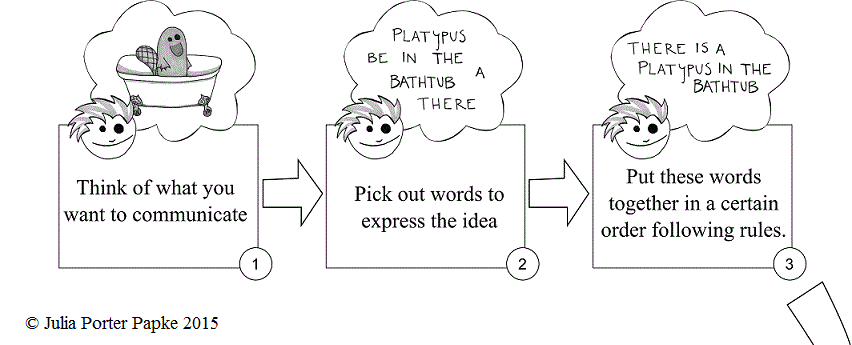
\includegraphics[width=1.0\textwidth]{img/speech-chain_01.png}    
    \end{center}
\end{frame}

\begin{frame}[t]{의사소통의 단계 (2/3)}
  \begin{center}
    단어의 발음을 떠올림 → 음성기관에 전달함 → 소리로 실현시킴
    \vfill
    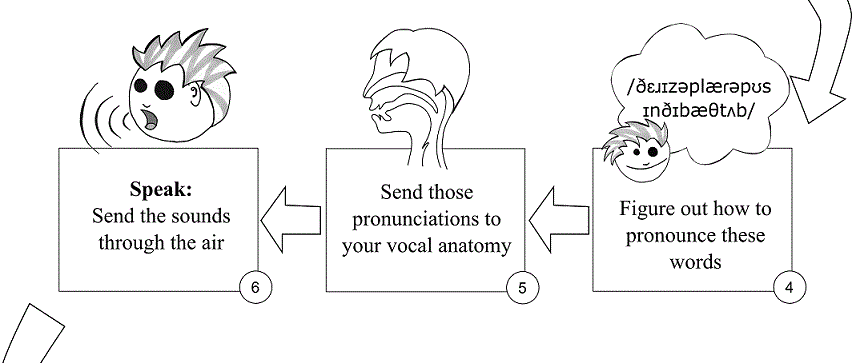
\includegraphics[width=1.0\textwidth]{img/speech-chain_02.png}
  \end{center}
\end{frame}

\begin{frame}[t]{의사소통의 단계 (3/3)}
  \begin{center}
    소리가 청자의 청각기관에 도달함 → 청자가 소리를 정보로 변환함 → 정보를 전달받음
    \vfill
    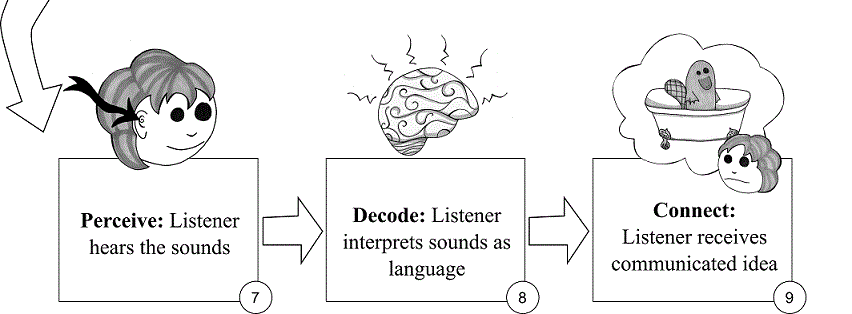
\includegraphics[width=1.0\textwidth]{img/speech-chain_03.png}
  \end{center}
\end{frame}

\begin{frame}[t]{의사소통의 단계적 연구}
    \begin{block}{주의!}
      이 모든 의사소통 단계에서, 화자/청자는 자기가 어떻게 그걸 하는지 설명하지 못함
    \end{block}  
    \begin{itemize}
      \item 이론언어학은 이 각각의 단계에 관여하는 지식들을 나누어서 연구함
      \item 형식과 내용을 나누어서 접근
    \end{itemize}

    \begin{columns}
      \begin{column}{0.5\textwidth}
        \begin{block}{형식(form)}
          \begin{itemize}
            \item 소리(음성학, 음운론)
            \item 단어의 형태(형태론)
            \item 문장의 구조(통사론)
          \end{itemize}
        \end{block}
        
      \end{column}
      \begin{column}{0.5\textwidth}
        \begin{block}{내용(meaning)}
          \begin{itemize}
            \item 단어의 의미(의미론)
            \item 문장의 의미(의미론)
            \item 문장의 맥락적 의미(화용론)
          \end{itemize}
        \end{block}
      \end{column}
    \end{columns}
\end{frame}

\begin{frame}[t]{의사소통의 단계적 연구}
    \begin{block}{음성학 (Phonetics)}
    \begin{itemize}
      \item \href{https://gongu.copyright.or.kr/gongu/wrt/wrt/view.do?wrtSn=13252844&menuNo=200020}{\underline{고양이 울음 소리}}와, 고양이 울음 소리를 흉내낸 [애오오옭 애오옭] 말소리를 구분할 수 있음
      \item 외국어의 말소리와 자기 언어의 말소리를 구분할 수 있음
      \item 자기 언어의 말소리를 발음할 수 있음
    \end{itemize}
  \end{block}

  \begin{block}{음운론 (Phonology)}
    \begin{itemize}
      \item ‘산’이 [과낙싼]에서는 [싼]으로 발음되고 [우리하꾜가인는산]에서는 [산]으로 발음되는 것을 알고 있음 
      \item 자기 언어에서 가능한 발음연속과 가능하지 않은 발음연속을 판단할 수 있음
      \item 다양한 사람에 의해 발음된 말소리를 ‘동일한 말소리’로 인식할 수 있음
    \end{itemize}
    
  \end{block}
\end{frame}

\begin{frame}[t]{의사소통의 단계적 연구}
  \begin{block}{형태론 (Morphology)}
    \begin{itemize}
      \item ‘과낙싸는서울시내와기오니달라요’과 같은 언어 표현을 ‘관악산은 서울 시내와 기온이 달라요’로 분절해서 인식할 수 있음
      \item ‘달라요’와 ‘다릅니다’가 ‘다르-’를 공유하고 있다는 것을 알고 있음
      \item ‘만들면’의 ‘-면’과 ‘먹으면’의 ‘-으면’이 다르지만 같은 표현이라는 것을 알고 있음
      \item ‘악플러’를 보고 ‘소비러’, ‘통학러’, ‘재수강러’ 등의 표현을 만들어낼 수 있음
      \item ‘출렁출렁’과 ‘우물쭈물’이 같은 방식으로 만들어진 단어임을 알고 있음
    \end{itemize}
  \end{block}
\end{frame}

\begin{frame}[t]{의사소통의 단계적 연구}
  \begin{block}{통사론 (Syntax)}
    \begin{itemize}
      \item ‘저번 때처럼 궁금해하지 말자’가 다음 두 문장에 대응할 수 있다는 것을 알고 있음
        \begin{itemize}
          \item ‘저번 때에 궁금해했고, 이번에는 그러지 말자’
          \item ‘저번 때에 궁금해하지 않았고, 이번에도 그러지 말자’
        \end{itemize}
        \vfill
      \item ‘저번 때처럼 궁금해하지 말자’를 다르게 말하는 법에 제한이 있다는 것을 알고 있음
        \begin{itemize}
          \item[\checkmark]‘궁금해하지 말자 저번 때처럼’
          \item[\texttimes] ‘궁금해하지 저번 때처럼 말자’
        \end{itemize}
        \vfill
      \item 영어에서 같은 ‘walk’를 주어에 따라 다르게 말해야 함을 알고 있음
        \begin{itemize}
          \item[\checkmark] ‘She walks’, ‘They walk’
          \item[\texttimes] ‘She walk’
        \end{itemize}
    \end{itemize}
  \end{block}
\end{frame}

\begin{frame}[t]{의사소통의 단계적 연구}
  \begin{block}{의미론 (Semantics)}
    \begin{itemize}
      \item ‘매트 위의 고양이’와 ‘고양이 위의 매트’가 서로 다른 상황을 가리킨다는 것을 알고 있음
      \item ‘매트 위의 고양이’와 ‘고양이 밑의 매트’가 동일한 상황을 가리킨다는 것을 알고 있음
      \item ‘뜨거운 아이스 아메리카노’가 이상하다는 것을 알고 있음
    \end{itemize}
  \end{block}
  \begin{center}
    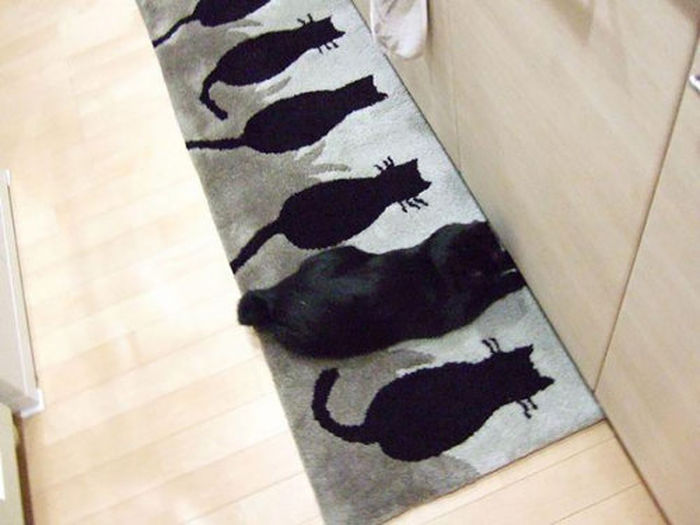
\includegraphics[width=0.4\textwidth]{img/fgvg8a60r5056otfhc05.jpg}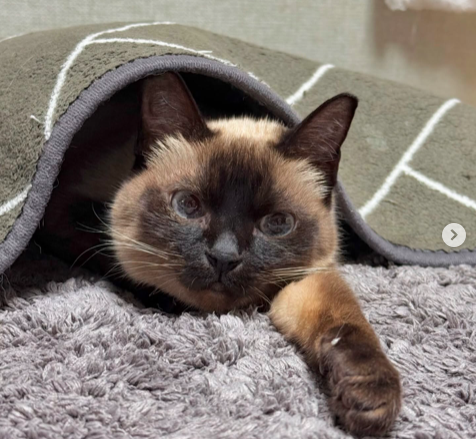
\includegraphics[width=0.32\textwidth]{img/mat_on_the_cat.png}
  \end{center}
\end{frame}

\begin{frame}[t]{의사소통의 단계적 연구}
  \begin{block}{화용론 (Pragmatics)}
    \begin{itemize}
      \item 좁은 통로에 서 있는 사람에게 ‘잠깐 지나갈 수 있을까요?’라고 물었을 때, ‘네’라고 대답한 채 움직이지 않으면 이상하다는 것을 알고 있음
      \item 다음 두 상황에서 ‘고소할거야’가 서로 다르다는 것을 알고 있음
        \begin{itemize}
          \item 운동하는데 트레이너가 엄살피우지 말래, 학대로 고소할거야
          \item 와 가만히 있는 사람을 쳤어? 폭행으로 고소할거야
        \end{itemize}
      \item 다음 말을 들었을 때 밥을 먹은 것이 전시를 보러 간 것보다 먼저라고 생각함
        \begin{itemize}
          \item 어제는 친구랑 밥을 먹고 전시를 보러 갔어
        \end{itemize}
    \end{itemize}    
  \end{block}  
\end{frame}

\begin{frame}[t]{언어 지식의 구성 요소}
  \begin{columns}
    \begin{column}[T]{0.5\textwidth}
      \begin{block}{어휘부(lexicon)}
        언어를 구성하는 단위들에 대한 지식
      \end{block}
    \end{column}
    \begin{column}[T]{0.5\textwidth}
      \begin{block}{규칙(rules)}
        언어를 구성하는 단위들이 결합하는 패턴에 대한 지식
      \end{block}
    \end{column}
  \end{columns}
  \begin{block}{언어 지식의 다른 명칭들}
    \begin{itemize}
      \item 문법(grammar): 어휘부와 규칙을 모두 포괄하는 언어 체계에 대한 지식
      \item 맥락에 따라서는 언어 = 언어 능력 = 언어 지식 = 문법
    \end{itemize}
  \end{block}
  \begin{block}{주의!}
    외국어 학습서의 \textbf{어휘}, \textbf{문법}과 혼동하지 말 것!
  \end{block}

\end{frame}

\section{언어와 관련된 다른 지식}

\begin{frame}[t]{쓰기 (Writing)}
  \begin{block}{특징}
    \begin{itemize}
      \item 언어를 소리 (또는 손짓) 이외의 물리적 매체로 표현하는 일
      \item 쓰기가 이루어지려면 생각이 소리 (또는 손짓)의 형식으로 먼저 고정되어야 함
      \item 의도적 학습 필요
      \item 뇌에서 말하기 영역과 동시에 다른 영역들도 사용됨
      \item 남에게 전달되기 전에 수정 가능
      \item 역사적으로 말하기보다 출현 시기가 더 늦음
    \end{itemize}
  \end{block}
  \begin{block}{참고}
    약 7,000개 언어 중 3,000개가 문자 없이 사용됨 (2019년 기준)
  \end{block}
\end{frame}

\begin{frame}[t]{규범 문법 vs. 기술 문법}
  \begin{block}{규범 문법(prescriptive grammar)}
    \begin{itemize}
      \item 사회적으로 규정/통용되는, 언어를 사용하는 \textbf{올바른} 방법
        \begin{itemize}
          \item \textasciitilde 라고 생각되어집니다 (X) vs. \textasciitilde 라고 생각합니다 (O)
          \item \textasciitilde 기 쉽상이다 (X) vs. \textasciitilde 기 십상이다 (O)
          \item 이빨을 들어내며 웃었다 (X) vs. 이빨을 드러내며 웃었다 (O)
        \end{itemize}
      \item 언어 사용 패턴들 중에서 \textbf{일부를 뽑아서} ‘올바름’의 가치를 부여
        \begin{itemize}
          \item ‘십상’을 ‘쉽상’으로 쓰는 것은 잘못되었다.
        \end{itemize}
      \item 대부분의 모어 화자들이 약간의 교육을 통해 잘 구사함
      \item 고정된 소수의 패턴
        \begin{itemize}
          \item 언어변화에 저항함(‘자장면’ vs. ‘짜장면’)
          \item 변이형을 갖지 않음(표준어 ‘부추’ vs. 방언 ‘부추, 본추, 부초, 분초, 푸추, 푼추’)
        \end{itemize}
      \item 언어 공동체의 유지에 기여함
    \end{itemize}    
  \end{block}
\end{frame}

\begin{frame}[t]{규범 문법 vs. 기술 문법}
  \begin{block}{기술 문법(descriptive grammar)}
    \begin{itemize}
      \item 언어의 사용 패턴을 파악하고자 하는 언어학의 연구 성과물
        \begin{itemize}
          \item 한국어에서 받침 ‘ㅇ’ 소리는 첫소리로 실현되지 않는다 
          \item 한국어에서 어떤 서술어는 ‘-는-’과 결합하지 않는다
          \item 한국어는 화자와 청자의 사회적 위계에 따라 표현이 달라질 수 있다
        \end{itemize}
      \item 모든 사용 패턴을 동등하게 취급
        \begin{itemize}
          \item 일부 한국어 화자들은 ‘십상’을 ‘쉽상’이라고 말한다.
        \end{itemize}
      \item 모어 화자들은 잘 모름
      \item 언어학 밖에서는 외국어로서의 XX어 교육 자료 개발시에 사용
        \begin{itemize}
          \item 초급 교재: 그런데, 그러니까
          \item 고급 교재: 근데, 그니까
        \end{itemize}
      \item 언어 능력의 탐구에 기여함
    \end{itemize}
  \end{block}  
\end{frame}

\section{언어의 특징}

\begin{frame}[t]{Hockett이 제시한 언어의 특징 (1/3)}
  \begin{block}{의사소통의 수단}
    언어수행으로 메시지를 발신하고 수신할 수 있음
  \end{block}
  \begin{block}{의미성(semanticity)}
    언어를 이루는 요소들은 의미 또는 기능을 지니고 있으며, 지닐 것으로 기대됨
  \end{block}
  \begin{block}{기능성(pragmatic function)}
    \begin{itemize}
      \item 언어수행으로 다른 개체의 행동에 영향을 줌
      \item 언어수행으로 다른 개체와의 관계에 영향을 줌
      \item 언어수행으로 주위를 파악하고 이해할 수 있음
    \end{itemize}
  \end{block}
\end{frame}

\begin{frame}[t]{Hockett이 제시한 언어의 특징 (2/3)}
  \begin{block}{교환성(interchangability)}
    언어 수행으로 메시지를 수신할 수도 있고 발신할 수도 있음
  \end{block}
  \begin{block}{문화적 전달(cultural transimission)}
    \begin{itemize}
      \item 다른 사람과의 접촉과 소통을 통해서 언어를 습득함
      \item 타인과의 접촉과 소통이 없으면 언어능력을 타고났어도 습득할 수 없음
      \item 타인과의 접촉과 소통에 사용된 바로 그 언어체계만을 습득함
    \end{itemize}
  \end{block}
  \begin{block}{자의성(arbitrariness)}
    언어의 형식(form)과 의미(meaning)는 무관하며 관행으로 연결되어 있을 뿐임
  \end{block}
\end{frame}

\begin{frame}[t]{Hockett이 제시한 언어의 특징 (3/3)}
  \begin{block}{분할성(discreteness)}
    \begin{itemize}
      \item 연속된 소리를 분절된 단위로 인식함
      \item 언어별로 다르지만 약 10개에서 100여개 정도의 단위 사용
      \item 작은 단위의 조합으로 더 큰 단위를 만들어냄
    \end{itemize}
  \end{block}
  \begin{block}{전위성(displacement)}
    \begin{itemize}
      \item ‘\textbf{지금}’ ‘\textbf{여기}’가 아닌 것을 다룰 수 있는 성질
      \item 존재하지 않는 대상에 대해서도 다룰 수 있음
    \end{itemize}
  \end{block}
  \begin{block}{생산성(productivity)}
    \begin{itemize}
      \item 새로운 메시지를 만들어냄
      \item 작은 단위로 만들어낼 수 있는 더 큰 단위에 제한이 없음
    \end{itemize}
  \end{block}
\end{frame}

\begin{frame}[t]{Hockett의 특징에 따른 언어 평가}
  \begin{block}{인간의 자연 언어 (9가지 특징을 모두 지님)}    
    \begin{tabular}{lcl}
    의사소통 수단 & O & 동료 개체와 의사를 주고받는 데 사용\\
    의미성 & O & 언어의 모든 요소가 의미를 지니고 있음 \\
    기능성 & O & 다른 개체를 움직일 수 있음\\
    교환성 & O & 발화할 수 있으면 수신할 수도 있음\\
    문화적 전달 & O & 다른 화자와 접하지 않으면 배우지 못함 \\
    자의성 & O & ‘나무’가 꼭 ‘나무’여야 할 필요는 없음\\
    분할성 & O & 분절된 말소리나 손짓으로 구성됨\\
    전위성 & O & 여기 없는 대상과 지금이 아닌 시간 등을 다룰 수 있음\\
    생산성 & O & 새로운 발화를 무한히 만들 수 있음
    \end{tabular}
  \end{block}  
\end{frame}

\begin{frame}[t]{Hockett의 특징에 따른 언어 평가}
  \begin{block}{인공언어: 파이썬}
    \begin{tabular}{lcl}
    의사소통 수단 & X & 컴퓨터와 의사소통을 하는 것은 아님\\
    의미성 & O & 파이썬 코드의 모든 요소가 의미를 지니고 있음\\
    기능성 & O & 컴퓨터에게 연산을 시킴\\
    교환성 & O & 코드를 읽을 수 있으면 쓸 수도 있음\\
    문화적 전달 & O & 타고나지 않으며 할 줄 아는 사람에게 배워야 함\\
    자의성 & O & 파이썬 코드 요소의 이름이 꼭 그 이름이어야 할 이유는 없음\\
    분할성 & O & 분절된 요소들로 구성됨\\
    전위성 & O & 존재하지 않는 데이터, 앞으로 실행될 함수 등을 지시할 수 있음\\
    생산성 & O & 새로운 코드를 무한히 짤 수 있음
    \end{tabular}
  \end{block}
\end{frame}

\begin{frame}[t]{Hockett의 특징에 따른 언어 평가}
  \begin{block}{동물의 언어: 돌고래의 의사소통 시스템}
    \begin{tabular}{lcl}
    의사소통 수단 & O & 음성 및 몸짓으로 동료 개체와 의사를 주고 받음\\
    의미성 & O & 고유한 개체를 가리키는 소리 확인됨\\
    기능성 & O & 먹이 사냥, 협력, 위험 경고, 놀이, 짝짓기 등에 사용\\
    교환성 & O & 음성/몸짓 신호를 보낼 수 있으면 받을 수도 있음\\
    문화적 전달 & O & 소리 일부는 교육되는 것이 확인됨 \\
    자의성 & ? & 증거 부족\\
    분할성 & ? & 증거 부족\\
    전위성 & ? & 증거 부족\\
    생산성 & ? & 증거 부족
    \end{tabular}
  \end{block}
\end{frame}

\begin{frame}[t]{Hockett의 특징에 따른 언어 평가}
  \begin{block}{곤충의 언어: 지렁이의 의사소통 시스템}
    \begin{tabular}{lcl}
    의사소통 수단 & O & 화학 신호 및 접촉으로 동료 개체와 의사를 주고 받음\\
    기능성 & O & 생존과 번식에 사용\\
    교환성 & O & 화학 신호 및 접촉 신호를 보낼 수 있으면 받을 수도 있음\\
    의미성 & X 또는 ? & '짝짓기 가능'을 의미로 볼 것인지에 따라 다름 \\
    문화적 전달 & X & 타고남 \\
    자의성 & X & 해당 개체의 번식 준비 상태와 필연적으로 연결됨, 사회적 약속 아님\\
    분할성 & X & 연속적 신호 사용, 분절 안 됨\\
    전위성 & X & 지금 여기의 상태에 대해서만 표현 가능\\
    생산성 & X & 정해진 몇 가지 신호만 반복
    \end{tabular}
  \end{block}
\end{frame}


\begin{frame}[t]{언어의 자의성}
  \begin{center}
    \begin{tikzpicture}
      % 개 그림 (간단한 표현)
      \draw[thick] (0,0) circle (0.5cm);
      \node at (0,0) {\LARGE\emoji{dog}};

      % 각 언어의 표현
      \node at (-4,-1.5) {한국어: 개};
      \node at (4,-1.5) {영어: dog};
      \node at (-2,-2.5) {일본어: 犬 (inu)};
      \node at (2,-2.5) {프랑스어: chien};

      % 화살표
      \draw[->] (-0.5,-0.5) -- (-3.5,-1.0);
      \draw[->] (0.5,-0.5) -- (3.5,-1.0);
      \draw[->] (-0.5,-0.5) -- (-1.5,-2.0);
      \draw[->] (0.5,-0.5) -- (1.5,-2.0);
    \end{tikzpicture}
  \end{center}

\begin{block}{자의성의 의미}
형식(form)과 의미(meaning)는 무관하며, 관행으로 연결됨  
\end{block}
흔한 ‘필연성’ 사고: ‘우리 뫄뫄는 어떻게 이름도 뫄뫄야’ 
\begin{itemize}
  \item 어떻게 이름도 ‘신동’주? 역대급 양궁 신동의 등장! 
  \item 고수는 어떻게 이름도 고수야..
\end{itemize}
\end{frame}

\begin{frame}[t]{언어의 자의성}
  \begin{block}{같은 뜻 다른 소리, 같은 소리 다른 뜻}
    \begin{center}
      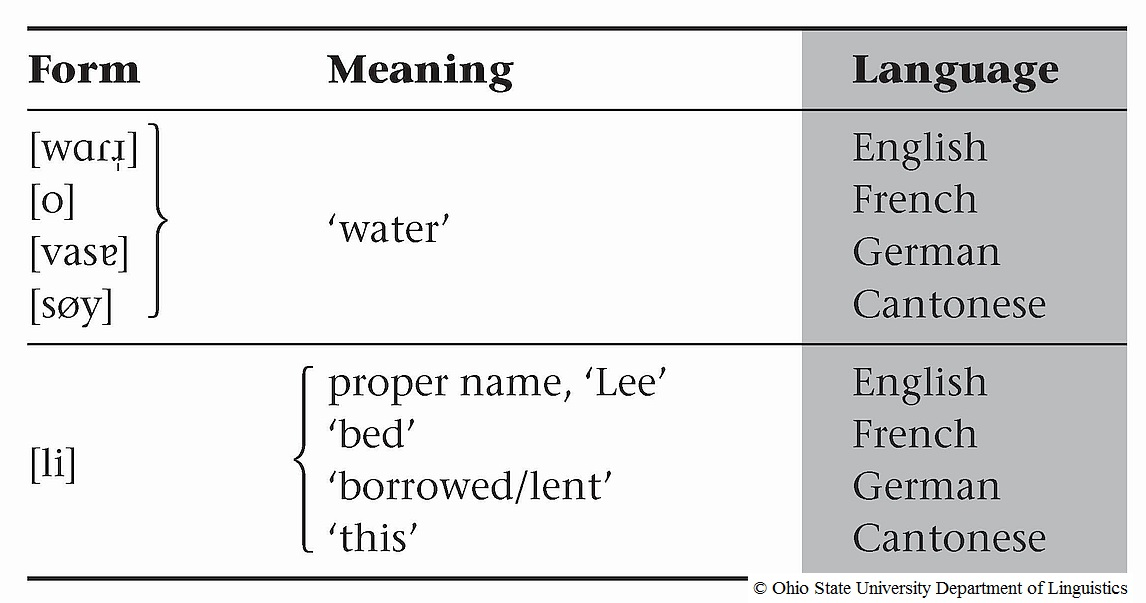
\includegraphics[width=0.8\textwidth]{img/form-meaning.jpg}        
    \end{center}
  \end{block}
\end{frame}

\begin{frame}[t]{언어의 자의성}
  \begin{block}{언어의 자의성에 대한 오해}
    “언제나 그 책상이 그 책상이구먼.”하고 그 남자는 중얼거렸다.\\
    “언제나 똑같은 책상, 언제나 똑같은 의자들, 똑같은 침대, 똑같은 사진이야. 그리고 나는 책상을 책상이라고 부르고 사진을 사진이라고 하고, 침대를 침대라고 부르지. 또 의자는 의자라고 한단 말이야. 도대체 왜 그렇게 불러야 하는 거지?” […]\\
    ‘왜 침대를 사진이라고 하면 안 되지?’ 그 남자는 이렇게 생각하면서 미소를 지었다. 그리고는 껄껄 웃기 시작했다. 옆방 사람이 벽을 두드리며 “거 좀 조용히 합시다.”하고 고함을 지를 때까지 그는 웃고 또 웃었다.\\
    “이제 모든 것이 달라질 거야.” 그는 이렇게 외치면서, 이제부터 침대를 ‘사진’이라고 부르기로 했다. “피곤하군, 이제 사진 속으로 들어가야겠어.”라고 말하고는 침대 위에 누웠다.\\
    - 《책상은 책상이다》, 페터 빅셀 지음
  \end{block}
\end{frame}

\begin{frame}[t]{언어의 ‘필연성’ 사고와 고대 그리스의 논쟁}
  \begin{block}{‘필연성’에 대한 부정}
    \setstretch{1.6} 헤르모네게스: \\ 
    저는 계약과 약속에 토대를 둔 것과는 다른 낱말들의 올바름이 존재한다는 것을 납득할 수 없습니다. 왜냐하면 저는 다음과 같이 생각하기 때문입니다. 누가 어떤 사물을 어떤 이름으로 부르게 되면, 그것이 올바른 이름이고, 다시금 다른 이름으로 대체하고 이전의 이름을 사용하지 않으면, 이것이 이전의 이름과 마찬가지로 올바른 것이 됩니다. […] 왜냐하면 사물의 이름은 본성으로부터 그 이름을 소유하는 것이 아니고, 낱말들을 만들고 사용하는 지시와 습관에 의해서 그 이름을 소유하게 되기 때문입니다.\\
    《크라튈로스: 명명의 올바름에 대하여》, 플라톤
  \end{block}
\end{frame}

\begin{frame}[t]{언어의 ‘필연성’ 사고와 고대 그리스의 논쟁}
  \begin{block}{‘필연성’에 대한 옹호}
    \setstretch{1.6} 소크라테스: \\ 
    우리가 인간이라고 부르는 것을 내가 말이라고 부르고, 말이라고 부르는 것을 인간이라고 부르면, 동일한 사물이 공적으로 사람으로 불리지만 내게는 특별히 말로서 불려지게 되고, 반대로 사람들에게는 공적으로 말로서 불리는 것이 내게 사람으로 불려져도 되는가? […] 즉 본성에 따른 적합한 도구를 만들어내야 하는 것일세. 이 일이 무엇에 의해서 만들어져야 하는지는 개별적인 의미에서가 아니라, 본성에 의한 것이네. \\
    《크라튈로스: 명명의 올바름에 대하여》, 플라톤
  \end{block}
\end{frame}


\section{언어 연구의 역사}

\begin{frame}[t]{언어 연구의 역사적 발전: 고대 그리스}
  \begin{block}{고전기 그리스의 외국어, 방언과 언어변화에 대한 인식}
      \begin{itemize}
        \item 고전기 그리스: 기원전 6세기부터 4세기까지의 그리스
        \item 그리스어와 다른 언어를 쓰는 이방인들(‘바르바로이’)에 대한 인식
        \item ‘하나의 언어를 쓰는 공동체로서의 그리스인’에 대한 인식 
        \item 호메로스의 《일리아드》와 《오디세이》의 언어가 당대의 어느 방언과도 일치하지 않는다는 사실에 대한 인식
      \end{itemize}
  \end{block}
  아테나이인들은 알렉산드로스에게 그렇게 말하는 한편 스파르테의 사절단에게는 다음과 같이 말했다. “우리가 페르시아 왕과 강화조약을 맺지 않을까 라케다이몬인들이 두려워하는 것은 당연한 일이오. [...] 우리는 모두 헬라스인들이오. 우리는 한 핏줄이고, 같은 말을 쓰고, 같은 신전을 사용하고, 같은 축제를 개최하며, 생활 방식 또한 같소이다. 아테나이인들이 이 모든 것을 배반한다는 것은 수치스런 짓이오. \\\\- 헤로도토스, 《역사》8권 144장, 천병희 역
\end{frame}

\begin{frame}[t]{언어 연구의 역사적 발전: 고대 그리스}
  \begin{block}{고전기 그리스의 문법 연구}
    \begin{itemize}
      \item 플라톤과 아리스토텔레스의 시대까지, 언어는 별도의 연구 분야로 인식되지 않음
      \item 소크라테스, 플라톤, 아리스토텔레스의 언어 분석: 철학의 일부로서 언어에 대한 고찰
    \end{itemize}
  \end{block}
  \begin{itemize}
    \item ‘그라마타(grámmata): 문자
    \item ‘그라마티코스(grammatikós)’: 문자를 이해하고 읽고 쓸 수 있는 사람
    \item ‘테크네 그라마티케(téchnē grammatik\texttnr{ḗ})’: 읽고 쓰기의 기술
  \end{itemize}
  \vfill
  \begin{itemize}
    \item 플라톤: 《크라튈로스(Cratylus)》
    \item 아리스토텔레스: 명제론, 범주론, 수사학, 시학 등 여러 저작에 흩어져 있는 언급들
  \end{itemize}
\end{frame}

\begin{frame}[t]{언어 연구의 역사적 발전: 고대 그리스}
  \begin{block}{헬레니즘 시대의 문법 연구}
    \begin{itemize}
      \item 그리스어와 그리스어 고전을 배우는 외국어 화자의 급증
      \item 코이네 그리스어의 등장
      \item ‘올바른’ 그리스어(=고전 그리스어)의 발음과 문법 지식에 대한 수요
    \end{itemize}
  \end{block}
  \begin{itemize}
    \item 스토아 학파의 언어 분석 → 언어학의 계통 1: 문법과 언어능력에 관한 탐구
    \item 알렉산드리아 학파의 언어 분석 → 언어학의 계통 2: 문법교육과 문학의 언어에 대한 탐구
  \end{itemize}
\end{frame}

\begin{frame}[t]{중세 유럽의 내성문법과 르네상스 이후의 언어관}
  \begin{block}{중세 유럽의 문법 연구}
    \begin{itemize}
      \item 내성문법/사변문법(speculative grammar) 연구
      \item 라틴어 문법 모형의 철학적 정당성의 탐구
      %   \begin{itemize}
      %     \item 명사: 계속 존재하는 것들
      %     \item 동사: 시간에 매인 일시적인 현상을 표현하는 것
      %   \end{itemize}
      % \item 언어와 인간 정신의 관계에 대한 탐구 
      \item 인간의 모든 언어에 보편적으로 존재하는 보편문법과 언어 보편소에 대한 탐구
    \end{itemize}    
  \end{block}
  \begin{block}{르네상스 \textasciitilde 19세기의 문법 연구}
    \begin{itemize}
      \item 유럽 사람들의 유럽 밖의 언어에 대한 탐색
      \item 유럽 내에서 개별 민족과 민족 언어를 의식하는 움직임
      \item 인쇄술이 발전하여 언어에 대한 지식을 서로 널리 공유
      \item 여러 언어의 문법을 기술하고 기준을 세워 비교하고 분류
    \end{itemize}
  \end{block}
\end{frame}

\begin{frame}[t]{19세기 유럽의 역사비교언어학 연구}
  \begin{block}{18세기 말, 윌리엄 존스의 연설}
    산스크리트어는 라틴어 및 그리스어와 너무나도 비슷해서, 아마도 지금은 존재하지 않는, 공통의 기원에서 자라나왔다고 생각하지 않을 수 없다
  \end{block}
  \begin{block}{19세기 독일 언어학자들}
    \begin{itemize}
      \item 그 언어들이 하나였다가 갈라져 나온 과정을 우리가 재구성할 수 있을까?
      \item 언어 연구가 ‘비교언어학’으로 독립함 
      \item 언어 변화의 양상과 원리를 분석하고 언어 변화 모형을 구축
    \end{itemize}
  \end{block}
\end{frame}

\begin{frame}[t]{구조주의 언어학, 생성문법, 그 이후}
  \begin{block}{19세기 말 \textasciitilde 20세기 초, 소쉬르}
    \begin{itemize}
      \item 언어의 개별 요소(및 그 변화) 연구만으로는 언어를 이해할 수 없다
      \item 언어 요소의 가치는 다른 요소와의 관계에서 생겨난다
      \item 사회적 실체로서의 ‘언어’(랑그)와 개인적 수행으로서의 ‘언어’(파롤) 구분
      \item 언어학의 연구 대상은 랑그
      \item 언어학의 연구 대상을 ‘특정 시기의 언어 상태’까지 확장
      \item 이후 1950년대까지 여러 언어를 대상으로 공시 문법 분석이 활발히 진행됨
    \end{itemize}
  \end{block}
\end{frame}

\begin{frame}[t]{구조주의 언어학, 생성문법, 그 이후}
  \begin{block}{20세기 중반, 촘스키}
    \begin{itemize}
      \item 이 모든 문법 구조들을 만들어내는 구조가 우리 마음 속에 있는 게 아닐까?
      \item 언어 능력: 언어를 이루는 구조들을 만들어낼 수 있는, 인간의 인지 구조
      \item 언어 수행: 언어 능력을 가지고 인간이 만들어내는 발화들
      \item 언어학의 연구 대상은 언어 능력
      \item 언어학의 영역을 인간의 인지 연구 분야로 확장시키는 데 기여함
    \end{itemize}
  \end{block}
\end{frame}

\begin{frame}[t]{구조주의 언어학, 생성문법, 그 이후}
  \begin{block}{20세기 후반의 언어학자들}
    \begin{itemize}
      \item 사람들의 언어 수행이 언어 구조와 무관하지 않은 것 같은데…?
      \item 언어 사용으로부터 언어 지식이 발생한다는 점에 대한 관심 - 사용 기반 이론의 발달
      \item 언어 사용 양상이 점진적으로 변화하면서 언어 변화가 일어난다는 관찰
      \item 인지언어학 등 새로운 이론틀의 등장
    \end{itemize}
  \end{block}
\end{frame}

\begin{frame}[t]{구조주의 언어학, 생성문법, 그 이후}
  \begin{block}{21세기 언어학}
    \begin{itemize}
      \item \textbf{다양한 이론틀의 공존}
        \begin{itemize}
          \item 생성문법
          \item 인지언어학
          \item 사용 기반 이론
        \end{itemize}
    \item \textbf{기술 발전의 활용}
        \begin{itemize}
          \item 대량 언어 자원 연구
          \item 컴퓨터 기반 분석
          \item 실험 언어학
        \end{itemize}
    \item \textbf{학제간 연구}
        \begin{itemize}
          \item 신경언어학
          \item 전산언어학
          \item 심리언어학
        \end{itemize}
    \end{itemize}    
  \end{block}
\end{frame}

\section{마무리}

\begin{frame}[t]{핵심 정리}
\begin{itemize}
\item 언어학은 개별 언어를 통해 보편적 언어 능력을 탐구한다
\item 언어는 체계적이고 과학적으로 연구할 수 있다
\item 언어 지식은 여러 층위로 구성된다(음성, 음운, 형태, 통사, 의미, 화용)
\item 언어 능력과 언어 수행의 구분이 중요하다
\item 언어는 자의적이지만 체계적이다
\item 언어학은 계속 발전하는 학문이다
\end{itemize}
\end{frame}

\begin{frame}[t]{참고문헌}
  \begin{itemize}
    \item \texttnr{Department of Linguistics, The Ohio State University (2022) \textit{Language Files}, 13th ed. Ohio State University Press. Chapter 1.}
    \item \texttnr{Robins, R. H. (1997) \textit{A Short History of Linguistics}, 4th ed. London and New York: Longman}
  \end{itemize}
\end{frame}

\end{document}